\documentclass[a4paper,11pt,onecolumn,oneside]{book}
\usepackage{amsfonts, amsmath, amssymb, amsthm}
\usepackage{graphics}
\usepackage{graphicx}
\usepackage[table]{xcolor}
\usepackage{dcolumn,multirow,longtable}
\usepackage{hyperref}
%\usepackage{subfigure}
\usepackage{float}
\usepackage{color}
\usepackage{colortbl}
\usepackage{caption}
\usepackage{perpage}
\usepackage{color}
\usepackage{graphicx}
\usepackage{subcaption} 
\MakeSorted{figure}
\MakeSorted{table}
%\usepackage{pst-all} % ps-tricks
%\usepackage[scanall]{psfrag}

% definition layout and print space
\setlength{\hoffset}{-1in}  
\setlength{\voffset}{-1in}         
\setlength{\topmargin}{2cm}      
\setlength{\oddsidemargin}{3cm}  
\setlength{\textwidth}{16cm}       
\setlength{\textheight}{23,4cm}    
\setlength{\headsep}{0.7cm}     

% theorems
\newtheorem{defi}{Definition}[chapter]
\newtheorem{prob}{Problem}
\newtheorem{alg}{Algorithm}
\newtheorem{rem}{Remark}
\newtheorem{prop}{Proposition}
\newtheorem{ex}{Example}
\newtheorem{theo}{Theorem}
\newcommand{\hilight}[1]{\colorbox{blue!30!}{#1}}



\begin{document}


\begin{titlepage}
\begin{center}
\textbf{\LARGE Management system for housing cooperative}\\ [2ex]\textbf{Computer Project Management }\\
[45ex]Ilona Brzozowska ID: 197006  \\ Pawel Glowacki ID: 196152 \\
 \hilight{Magdalena Ronge ID:195753} \\ Krystian Sulinski ID: 190585 \\
{\today} \\
[70ex]{Wroclaw University of Technology} \\
\end{center}
\end{titlepage}

\tableofcontents

\chapter{Project description}

\section{The Purpose of the Project}



\subsection{The User Business or Background of the Project Effort}

Our client - AppartMeans, aim to build housing estate, which needs housing cooperative software
system. In order to this new enterprise, AppartMeans sign alignment with housing cooperative
which has not used any software up to now. The software which needs to be developed should
enable full communication between housing cooperative and new residents to make AppartMeans
housing estate more modern and residents friendly. The board of AppartMeans decided to
improve customers satisfaction by providing website application for residents. The quality of
customers satisfaction should be measure of the time spending every month in our application.



\subsection{Goals of the Project}

The main goal is project and implementation of database application for purpose of account
management by housing association. Final product will be consist of two main parts: web
application (for residents) and desktop application (for administration). These applications
assure of:


\begin{itemize}
 
  \item Remove necessity face to face contact between house cooperative and resident
  \item  Automated and error-free calculating of bills
  \item Provide up-to-date flow of information between sides
  \item Enable review of all already paid bills, media usage and its price in every month
  \item Make the billing process paperless

\end{itemize}

Final applications should allow its users to do as much as possible things related with paying bills and communication, but should do it more friendly and less time-consuming. Residents should use our service because it simplifies managing their bills management, not because they have to. Therefore measure of success should be the time they are spending on functionalities not obligatory to them, like checking the history of bills or media usage instead of checking them manually.

\section{The Stakeholders}

\subsection{The Client}
The client can be either housing cooperatives,  house developer or house rental company. Our client is company AppartMeans whitch sign alignment with housing cooperative.

\subsection{Other Stakeholders}

\begin{enumerate} 
\item \textbf{Customers and users as a stakeholders} - Because housing management system will provide such functionality as gathering bills data, it is necessary to consult project with media suppliers (water, power, gas). The structure of each type of bill is essential for correct  accounting.
On the other hand, there is a certain need to consult project with future users. For example for establishing requirements for user functionality.


\item \textbf{People involved in developing product:}
\begin{itemize}
	\item Testers
	\item Developers
	\item System and database architects
	\item Domain specialist (people who knows housing industry)
	\item Sponsors
\end{itemize}
\end{enumerate}

\subsection{The Hands-On Users of the Product}
\begin{enumerate}
	\item  \textbf{Tenants} –  they will have possibilities to improve bills management. First of all – browsing bills, according to their date, type (water, power etc.). Moreover there will be functionality allowing to generate charts and figures based on bills. As a result user obtains graphical representation of his bills – how much he pays for particular medium in previous months or for example what is the share of gas bills in overall cost in current month.
            	In addition they will manage their own accounts (changing e-mails, password, sending/receiving messages).

	\item  \textbf{Housing administration} – apartments owner (not only person, but also company), who manages the system. He has privileges to add/remove users(tenants) and buildings he owns. For improving communications, he will send messages and notifications to tenants (for example about formal meeting, some reminders etc.). An administrator will be a person, who inputs the data about the bills.
\end{enumerate}

\subsection{Personas}

Management of houses rental company is a huge-scoped task.  That leads to partition of administrative duties. 
\begin{itemize}
\item \textbf{Administrator in terms of entire system} - it means a person who will be dealing with database management and maintaining the system. He will focus on technical aspects of system.
\item Second group will be textbf{administrative employees} – they will be involve in billing the tenants and delivering them various information, e.g. meetings, renovations . They needs to be familiar with system’s main functionalities, so probably there will be a need of special user training for them.
The separate user group will be tenants. Just people interested in making their lives easier by using e-system that allows to monitor and analyze their mortgage, bills. If one of housing agency goal will be mandatory use of the system, there should be a special user training also for the tenants.
\end{itemize}


\subsection{Priorities Assigned to Users}

The goal of using housing management system is to simplify the business activities of owners. They need to have a practical tool that will fulfill that goal. Because they are customers and “customer is always right”, they will be the most important users. The feedback of housing administration will determine if the project is useful and in the end – successful.
On the other hand – tenants attitude to user application will be very important. Simple and user-friendly interface, helpful functionalities – that will be the factor that will draw their attention.


\subsection{User Participation}

As a result of previous description and a fact, that success of this project depends on customers and users satisfaction, the research of their needs should be done. Many functionalities may be implemented after consults with them.
It is especially important, because different housing cooperatives can have different needs. It may appear, that some functionalities should be implemented as a exchangeable plug-ins.


\subsection{Maintenance Users and Service Technicians}

In order to ensure system stability and high service availability, system admin will provide software maintenance. On the other hand company itself should hire technician (if they decide to maintain their own hardware) and database administrator or person responsible for data maintenance. Of course it can be avoided by provide them such kind of service.
Database administration can be provided by OUR company as a part of helpdesk.



\section{Mandated Constraints}
\subsection{Solution Constraints}

The project should be done in programming language named \texttt{C\#} using .NET framework in order to assure neat and minimalist interface – because of embedded well-designed libraries. Accordingly it is necessary to use Model View Controller for Web Application and Windows Presentation Foundation for Desktop Application.

To insure excellent quality of our software from the very beginning of programming, we are going to work in Test-Driven Development. All this work will be organizing in Microsoft Visual Studio. This is very popular IDE facilitates quick start and reliable during work.

\subsection{Implementation Environment of the Current System}

Administration of Council House has up to now three PC’s. We have to assure access to external providers (like gas and water provide) and create local database (Internal server at Figure \label{fig:rys1}).

The council house consist of two buildings, where are dwell residents. They hold a connection between Administration of Council House by Server, which is encrypted from two sided.

 \begin{figure}[H]
    \centering
            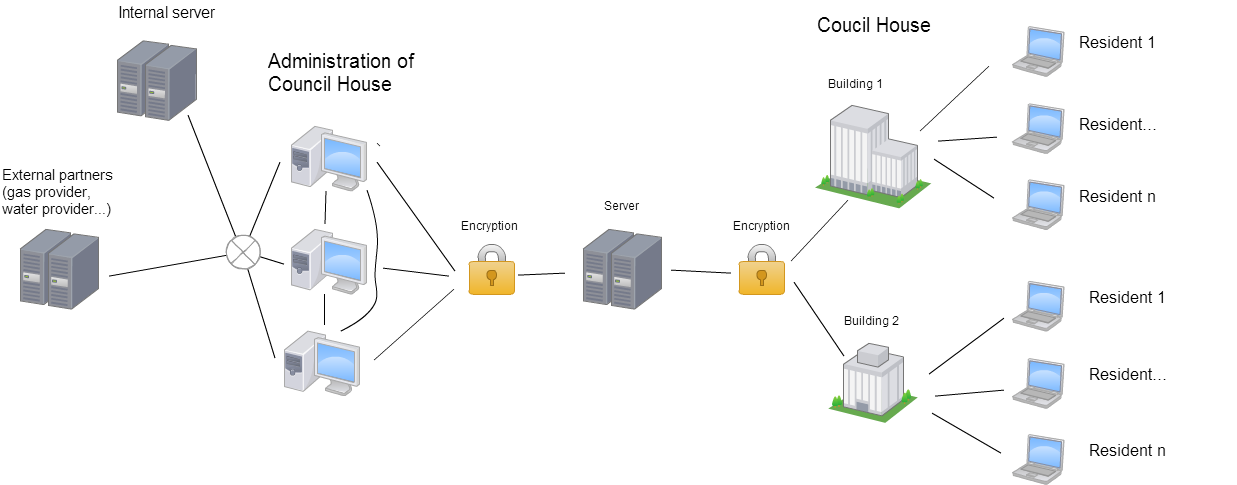
\includegraphics[width=1\textwidth]{img/diagramofinterfaces.png}
    \caption{Implementation Environment}
\label{fig:rys1}
\end{figure} 

\subsection{Partner or Collaborative Applications}

Our software will has to collaborate with i.a. gas and water provider. Their interfaces are not known so far.

\subsection{Off-the-Shelf Software}

To implements some of the requirements for the product we have to use some open source software mentioned in 3a. Solution Constraints – like Microsoft Visual Studio or .NET frameworks.


\subsection{Anticipated Workplace Environment}

The end users of our applications are residents of council house. Thus they will be work and use this product in their flats. The power sockets are in all the flat, but we know close to nothing about computer equipment of the residents. The workplace of Administration of Council House is located in a few rooms. The required source of power and Internet are provided.

\subsection{Schedule Constraints}

This project starts on 10th March 2015 and ends 20th July 2015.
Tasks are dived on 5 types, which every of them has its own deadline.
Accurate state deadline limitations are given at the table below.


\begin{table}[H]
\centering
\begin{tabular}{|l|l|l|l|}
\hline
\rowcolor{pink}\multicolumn{1}{|c|}{\textbf{Task Name}} & \multicolumn{1}{c|}{\textbf{Duration}} & \multicolumn{1}{c|}{\textbf{Start}} & \multicolumn{1}{c|}{\textbf{Finish}} \\ \hline
\textbf{\begin{tabular}[c]{@{}l@{}}1.\\   requirements\end{tabular}} & \begin{tabular}[c]{@{}l@{}}10\\   days\end{tabular} & \begin{tabular}[c]{@{}l@{}}Tue\\   15-03-10\end{tabular} & \begin{tabular}[c]{@{}l@{}}Mon\\   15-03-23\end{tabular} \\ \hline
talking with clients & 5 days & \begin{tabular}[c]{@{}l@{}}Tue\\   15-03-17\end{tabular} & \begin{tabular}[c]{@{}l@{}}Mon\\   15-03-23\end{tabular} \\ \hline
preparing documentations & 10 days & \begin{tabular}[c]{@{}l@{}}Tue\\   15-03-10\end{tabular} & \begin{tabular}[c]{@{}l@{}}Mon\\   15-03-23\end{tabular} \\ \hline
\textbf{2. design} & \begin{tabular}[c]{@{}l@{}}20\\   days\end{tabular} & \begin{tabular}[c]{@{}l@{}}Tue\\   15-03-24\end{tabular} & \begin{tabular}[c]{@{}l@{}}Mon\\   15-04-20\end{tabular} \\ \hline
database & 10 days & \begin{tabular}[c]{@{}l@{}}Tue\\   15-03-24\end{tabular} & \begin{tabular}[c]{@{}l@{}}Mon\\   15-04-06\end{tabular} \\ \hline
application's interface & 10 days & \begin{tabular}[c]{@{}l@{}}Tue\\   15-04-07\end{tabular} & \begin{tabular}[c]{@{}l@{}}Mon\\   15-04-20\end{tabular} \\ \hline
\textbf{\begin{tabular}[c]{@{}l@{}}3.\\   implementation\end{tabular}} & \begin{tabular}[c]{@{}l@{}}30\\   days\end{tabular} & \begin{tabular}[c]{@{}l@{}}Tue\\   15-04-21\end{tabular} & \begin{tabular}[c]{@{}l@{}}Mon\\   15-06-01\end{tabular} \\ \hline
\textbf{\begin{tabular}[c]{@{}l@{}}3.1\\   primary features\end{tabular}} & \begin{tabular}[c]{@{}l@{}}20\\   days\end{tabular} & \begin{tabular}[c]{@{}l@{}}Tue\\   15-04-21\end{tabular} & \begin{tabular}[c]{@{}l@{}}Mon\\   15-05-18\end{tabular} \\ \hline
logging & 5 days & \begin{tabular}[c]{@{}l@{}}Tue\\   15-04-21\end{tabular} & \begin{tabular}[c]{@{}l@{}}Mon\\   15-04-27\end{tabular} \\ \hline
admin's management & 5 days & \begin{tabular}[c]{@{}l@{}}Tue\\   15-04-28\end{tabular} & \begin{tabular}[c]{@{}l@{}}Mon\\   15-05-04\end{tabular} \\ \hline
browsing bills & 5 days & \begin{tabular}[c]{@{}l@{}}Thu\\   15-04-23\end{tabular} & \begin{tabular}[c]{@{}l@{}}Wed\\   15-04-29\end{tabular} \\ \hline
\textbf{\begin{tabular}[c]{@{}l@{}}3.2\\   secondary features\end{tabular}} & \begin{tabular}[c]{@{}l@{}}10\\   days\end{tabular} & \begin{tabular}[c]{@{}l@{}}Mon\\   15-05-18\end{tabular} & \begin{tabular}[c]{@{}l@{}}Fri\\   15-05-29\end{tabular} \\ \hline
sending bills to users & 5 days & \begin{tabular}[c]{@{}l@{}}Mon\\   15-05-18\end{tabular} & \begin{tabular}[c]{@{}l@{}}Fri\\   15-05-22\end{tabular} \\ \hline
sending notifications & 5 days & \begin{tabular}[c]{@{}l@{}}Mon\\   15-05-25\end{tabular} & \begin{tabular}[c]{@{}l@{}}Fri\\   15-05-29\end{tabular} \\ \hline
\textbf{4. testing} & \begin{tabular}[c]{@{}l@{}}15\\   days\end{tabular} & \begin{tabular}[c]{@{}l@{}}Mon\\   15-06-01\end{tabular} & \begin{tabular}[c]{@{}l@{}}Fri\\   15-06-19\end{tabular} \\ \hline
integration testing & 7 days & \begin{tabular}[c]{@{}l@{}}Mon\\   15-06-01\end{tabular} & \begin{tabular}[c]{@{}l@{}}Tue\\   15-06-09\end{tabular} \\ \hline
system testing & 7 days & \begin{tabular}[c]{@{}l@{}}Wed\\   15-06-10\end{tabular} & \begin{tabular}[c]{@{}l@{}}Thu\\   15-06-18\end{tabular} \\ \hline
acceptance testing & 1 day & \begin{tabular}[c]{@{}l@{}}Fri\\   15-06-19\end{tabular} & \begin{tabular}[c]{@{}l@{}}Fri\\   15-06-19\end{tabular} \\ \hline
\textbf{\begin{tabular}[c]{@{}l@{}}5.\\   maintenance\end{tabular}} & \begin{tabular}[c]{@{}l@{}}21\\   days\end{tabular} & \begin{tabular}[c]{@{}l@{}}Mon\\   15-06-22\end{tabular} & \begin{tabular}[c]{@{}l@{}}Mon\\   15-07-20\end{tabular} \\ \hline
getting feedback & 10 days & \begin{tabular}[c]{@{}l@{}}Mon\\   15-06-22\end{tabular} & \begin{tabular}[c]{@{}l@{}}Mon\\   15-07-13\end{tabular} \\ \hline
fixing bugs & 5 days & \begin{tabular}[c]{@{}l@{}}Tue\\   15-07-14\end{tabular} & \begin{tabular}[c]{@{}l@{}}Mon\\   15-07-20\end{tabular} \\ \hline
\end{tabular}
\caption{Deadlines}
\label{tab:dwadlines}
\end{table}

If we do not build the product by the end of the July, we have to contact with our client to set new dates.  

The financial impact of not having the product by the beginning of 2016 will be cost us 50\% price of this product.

\subsection{Budget Constraints}

The budget for the project is 100 000 PLN. There are 7 persons included, which overall predicted effort is about 1 500 hours. Is is required to obtain two laptops and assure catering.

\subsection{Enterprise Constraints}

There are 7 persons which can create this project. If the deadlines will be exceeded, we are obliged to hire at least one more person. These people can work at most 12 work a day, but no longer than for 3 days in a row. Standard work time is 8 days a day, but some of us work in another projects as well.


\section{Naming Conventions and Terminology}
\subsection{Glossary of All Terms, Including Acronyms, Used by Stakeholders involved in the Project}
This glossary will be extended throughout the project.



\begin{table}[H]
\begin{tabular}{p{5cm}p{9cm|}}
\hline
\rowcolor{pink}\multicolumn{1}{|c|}{\textbf{term}} & \multicolumn{1}{c|}{\textbf{definition}} \\ \hline
\textit{\textbf{project}} & \begin{tabular}[c]{@{}l@{}}doing all the things in order to obtain desired\\   software\end{tabular} \\ \hline
\textit{\textbf{council house}} & a group of buildings where are dwell residents \\ \hline
\textit{\textbf{resident}} & \begin{tabular}[c]{@{}l@{}}an end-user, which live in a building, which\\   belongs to council house\end{tabular} \\ \hline
\textit{\textbf{administration of council house}} & all the people which will be maintain ant provide up-to-date content of the database and contact with residents\ \\ \hline
\textit{\textbf{team leader}} & \begin{tabular}[c]{@{}l@{}}project manager, the person which take\\   responsibility for contact with client\end{tabular} \\ \hline
\textit{\textbf{primary features}} & \begin{tabular}[c]{@{}l@{}}all the features which has to be mandatory\\   provided\end{tabular} \\ \hline
\textit{\textbf{secondary features}} & \begin{tabular}[c]{@{}l@{}}all the features which can be optionally\\   provided\end{tabular} \\ \hline
\end{tabular}
\end{table}

\section{Relevant Facts and Assumptions}
\subsection{Relevant Facts}

\begin{enumerate}
\item \textbf{Accounting bills} is a functionality realized by housing cooperative owner. In fact, he may not receive all the bills, so there should be a possibility to make an agreement with e.g. power provider and use their API.
\item \textbf{Security of personal data} should be considered. Personal and business information of tenants are confidential – every use of them in the system should be legal.
\end{enumerate}

\subsection{Business Rules}

Company willingness of using this product is only a small part of way to success. Also the future users (tenants) should be satisfied.

\subsection{Assumptions}

\begin{itemize}
\item  Software for users should be system independent. Good way to achieve this is to realize client interface as a web service.
\item The final product will be still developed after finalizing the transaction. It is very important to make this kind of software up-to-date.
\item Any major changes will be consulted with current customers.
\item Because the project scope is dependent on client will, the most of functionalities should be implemented as a plug-ins.


\end{itemize}

\section{The Scope of the Work}
\subsection{The Current Situation}

Existing business processes are mainly manual so there is a need 
to automate process of sending, analysing and managing of bills, 
improvement of system of making announcements regarding community is 
also demanded. Currently, there is few people attempting surveys and 
voting, making the process easier will make people more cooperative.


\subsection{The Context of the Work}

 \begin{figure}[H]
    \centering
            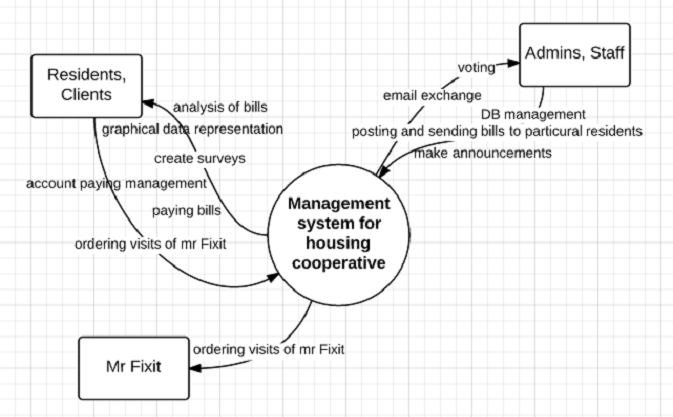
\includegraphics[width=1\textwidth]{img/paw1d.png}
\label{fig:rys1}
\end{figure} 

\subsection{Work Partitioning}
1:
\begin{itemize}
\item event: analysis of bills
\item input: user data
\item output: information about user's bills
\end{itemize}
2:
\begin{itemize}
\item event: account paying management
\item input: payments
\item output: information about user's bills

\end{itemize}
3:
\begin{itemize}
\item event: database management
\item input: create/remove user/building
\item output: updated database 
 
\end{itemize}
4:
\begin{itemize}
\item event: posting and sending bills to particular residents
\item input: resident's data
\item output: bills
 
\end{itemize}
5:
\begin{itemize}
\item event: make announcements regarding community
\item input: announcement
\end{itemize}
6:
\begin{itemize}
\item event: create surveys
\item input: question, options
\item output: survey

\end{itemize}
7:
\begin{itemize}
\item event: paying bills
\item input: payment
\item output: updated account balance 
\end{itemize}
8:
\begin{itemize}
\item event: graphical data presentation
\item input: user's account data
\item output: graph

\end{itemize}
9:
\begin{itemize}
\item event: converting graphs into .pdf format
\item input: graph
\item output: .pdf

\end{itemize}
10:
\begin{itemize}
\item event: ordering visits of Mr Fixit
\item input: information about fault
\item output: Mr Fixit's notification
\end{itemize}


\section{Business Data Model and Data Dictionary}
\subsection{Business Data Model}

 \begin{figure}[H]
    \centering
            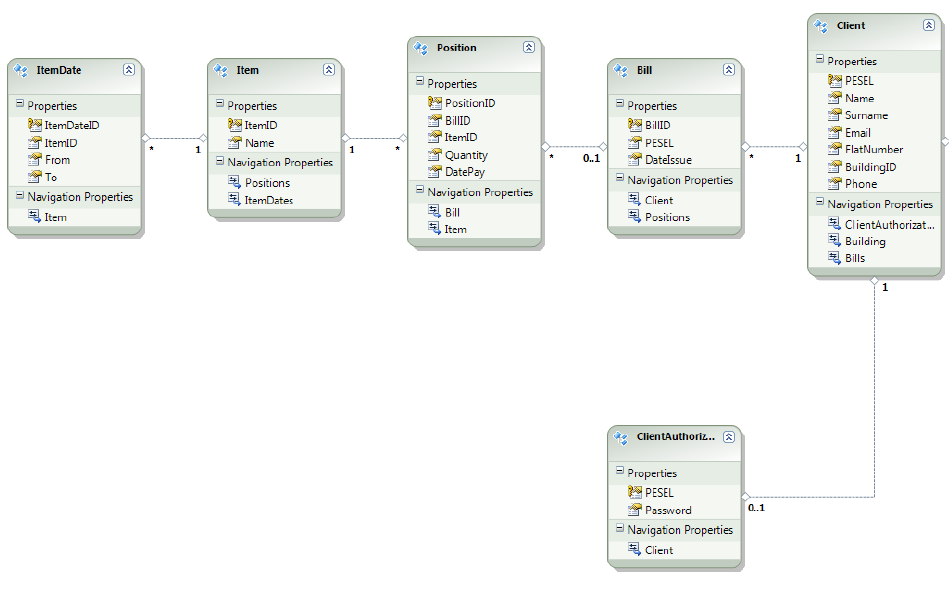
\includegraphics[width=1\textwidth]{img/databaseModel.png}
                \caption{Database model}
\label{fig:rys1}
\end{figure} 

\subsection{Data Dictionary}

\begin{table}[H]
\begin{tabular}{|l|l|l|l|}
\hline
\rowcolor{pink}\textbf{Data Name}  & \textbf{Description}                                                                                                & \textbf{Definition}                                                    & \textbf{Data Type} \\ \hline
Client              & \begin{tabular}[c]{@{}l@{}}a resident which \\ lives in a building\end{tabular}                                     & client name                                                            & Class              \\ \hline
Building            & \begin{tabular}[c]{@{}l@{}}a place where \\ client lives\end{tabular}                                               & \begin{tabular}[c]{@{}l@{}}exact address of \\ a building\end{tabular} & Class              \\ \hline
Bill                & \begin{tabular}[c]{@{}l@{}}an amount of \\ money which client \\ has to pay,\\   f.e. for gas or water\end{tabular} & amount of money                                                        & Class              \\ \hline
Position            & \begin{tabular}[c]{@{}l@{}}a concrete bill with \\ defined amount of money\\   and the kind of bill\end{tabular}    & \begin{tabular}[c]{@{}l@{}}bill position + \\ item ID\end{tabular}     & Class              \\ \hline
Item                & an item of a bill                                                                                                   & item ID + name                                                         & Class              \\ \hline
ItemDate            & a date of a item                                                                                                    & itemDateID + name                                                      & Class              \\ \hline
ClientAuthorization & \begin{tabular}[c]{@{}l@{}}date need to authorize \\   a client\end{tabular}                                        & PESEL + password                                                       & Class              \\ \hline
\end{tabular}
\end{table}

\section{The Scope of the Product}
\subsection{Product Boundary}
 \begin{figure}[H]
    \centering
            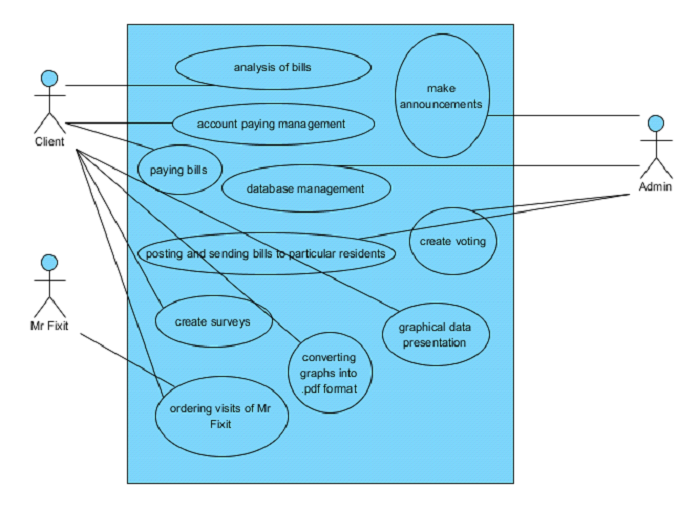
\includegraphics[width=1\textwidth]{img/paw2.png}
                \caption{Use Case Table}
\label{fig:rys1}
\end{figure} 

\subsection{Product Use Case Table}
\begin{itemize}
\item PUC Name: analysis of bills,
input: user data,
output: information about user's bills,
actor: client.

\item PUC Name: account paying management,
input: payments,
output: information about user's bills,
actor: client.

\item PUC Name: database management,
input: create/remove user/building,
output: updated database,
actor: administrator.

\item PUC Name: posting and sending bills to particular residents,
input: resident's data,
output: bills,
actor: administrator.

\item PUC Name: make announcements regarding community,
input: announcement,
actor: administrator.

\item PUC Name: create surveys,
input: question, options,
output: survey,
actor: client.

\item PUC Name: paying bills,
input: payment,
output: updated account balance,
actor: client.

\item PUC Name: graphical data presentation,
input: user's account data,
output: graph,
actor: client.

\item PUC Name: converting graphs into .pdf format,
input: graph,
output: .pdf,
actor: client.

\item PUC Name: ordering visits of Mr Fixit,
input: information about fault,
output: Mr Fixit's notification,
actor: client, Mr Fixit.

\item PUC Name: create voting regarding expenses of community, 
input: question, options,
output: voting,
actor: client, administrator.

\item PUC Name: e-mails exchange between collective’s administration and their residents, 
input: email addresses,
output: possibility to communicate,
actor: administrator, client.
\end{itemize}

\subsection{Individual Product Use Cases (PUC’s)}

\begin{itemize}
\item PUC Name: analysis of bills
\item Scenario: Client wants to check details about his bills. He can access to it.


\item PUC Name: account paying management
\item Scenario: Client needs to pay bills. He can do it. Client can access to history of payments.

\item PUC Name: database management
\item Scenario: New building has been built/removed. New resident has moved in/out. Administrator updates data in database.

\item PUC Name: posting and sending bills to particular residents
\item Scenario: There is a need to send bills to particular residents. Administrator does it.

\item PUC Name: make announcements regarding community
\item Scenario: There is a need to notify residents about something. Administrator makes announcement and residents can read it.

\item PUC Name: create surveys
\item Scenario: There is a need to decide about something. Decision depends on resident's opinion. Survey is created, residents can vote.

\item PUC Name: paying bills
\item Scenario: Client needs to pay bills. He can do it.

\item PUC Name: graphical data presentation
\item Scenario: Client wants to see data in graphical representation. Graph is displayed.

\item PUC Name: converting graphs into .pdf format
\item Scenario: Some clients prefers format pdf. Graph is converted.

\item PUC Name: ordering visits of Mr Fixit
\item Scenario: There is a fault in the building. Client orders visit of Mr Fixit. Mr Fixit get a message and come to repair fault.

\item PUC Name: create voting regarding expenses of community 
\item Scenario: There is a need to decide about something. Decision depends on resident's opinion. Survey is created, residents can vote.

\item PUC Name: e-mails exchange between collective’s administration and their residents.
\item Scenario: Residents can't communicate with administration during office hours. They can email them via application.
Administration can't meet a resident in reference to something. So they can email resident.

\end{itemize}

\chapter{Functional Requirements}



% Mandatory requirement  Mandatory requirement  Mandatory requirement  Mandatory requirement
%%%%%%%%%%%%%%%%%%%%%%%%%%%%%%%%%%%%%%%%%%%%%%%%
\section{Mandatory requirements}


\begin{table} [H]
%1
\centering
\begin{tabular} {p{5cm}p{9cm}} \\ \hline
\rowcolor{blue!20!black!30!green}\multicolumn{2}{|c|}{Mandatory requirement 1} \\ \hline
Description  & The system for administrator shall provide ability of adding and deleting users. \\ \hline
Rationale  & To be able to add and delete residents of new estate by name (if resident of given apartment will change, the old might be deleted and new resident added). It will allow administrator to keep information about bills private (old residents won’t have access to bills).  \\ \hline
Originator & Magdalena Ronge - Software Engineer\\ \hline
Fit Criterion & Signed users shall always match the real appartment residents. Separate accounts allows users identification. \\ \hline
Customer Satisfaction & 6/10\\ \hline
Customer Dissatisfaction & 9/10\\ \hline
Dependendies & A requirement providing adding and deleting buildings. \\ \hline

\end{tabular}
\label{tab:params}
\end{table} 

\begin{table} [H]

%2
\centering
\begin{tabular}{p{5cm}p{9cm}}  \hline
\rowcolor{blue!20!black!30!green}\multicolumn{2}{|c|}{Mandatory requirement 2} \\ \hline
Description  & The system for administrator shall provide ability to adding and deleting buildings\\ \hline
Rationale  & To be able to add and delete buildings and apartments by unique address. It will allow administrator expand activity in case of new estates. \\ \hline
Originator & Pawel Glowacki - Software Enineer\\ \hline
Fit Criterion & Signed buildings allows for apartments identification.\\ \hline
Customer Satisfaction & 6/10\\ \hline
Customer Dissatisfaction & 8/10\\ \hline
Dependendies & A requirement providing adding and deleting users (which will be assigned to buildings and apartments). \\ \hline

\end{tabular}
\label{tab:params}
\end{table} 

%3
\begin{table} [H]

\centering
\begin{tabular}{p{5cm}p{9cm}}  \hline
\rowcolor{blue!20!black!30!green}\multicolumn{2}{|c|}{Mandatory requirement 3} \\ \hline
Description  & The system for administrator shall provide ability of assigning users to buildings.\\ \hline
Rationale  & For house cooperative to have all information about all residents in buildings and apartments.  Help to manage whole estate.\\ \hline
Originator &  Pawel Glowacki - Software Enineer\\ \hline
Fit Criterion & Specific apartment shall match the user (by user ID, name and surname). \\ \hline
Customer Satisfaction & 6/10\\ \hline
Customer Dissatisfaction & 8/10\\ \hline
Dependendies & A requirement providing adding and deleting users (mandatory requirement 1) and a requirement providing adding and deleting building (mandatory requirement 2).\\ \hline

\end{tabular}
\label{tab:params}
\end{table} 

%4
\begin{table} [H]

\centering
\begin{tabular}{p{5cm}p{9cm}}  \hline
\rowcolor{blue!20!black!30!green}\multicolumn{2}{|c|}{Mandatory requirement 4} \\ \hline
Description  & The system for administrator shall provide list of buildings.\\ \hline
Rationale  & List view is clearer and makes searching process less time.\\ \hline
Originator &  Pawel Glowacki - Software Enineer\\ \hline
Fit Criterion & Administrator shall be able to find building or group of buildings in relatively shorter time.\\ \hline
Customer Satisfaction & 5/10\\ \hline
Customer Dissatisfaction & 7/10\\ \hline
Dependendies & A requirement providing adding and deleting buildings (mandatory requirement 2). \\ \hline

\end{tabular}
\label{tab:params}
\end{table} 

%5
\begin{table} [H]

\centering
\begin{tabular}{p{5cm}p{9cm}}  \hline
\rowcolor{blue!20!black!30!green}\multicolumn{2}{|c|}{Mandatory requirement 5} \\ \hline
Description  & The system for administrator shall provide list of users. \\ \hline
Rationale  & List view is clearer and makes searching process less time. \\ \hline
Originator &  Pawel Glowacki - Software Enineer\\ \hline
Fit Criterion & Administrator shall be able to find user or group of users in relatively shorter time.\\ \hline
Customer Satisfaction & 5/10\\ \hline
Customer Dissatisfaction & 7/10\\ \hline
Dependendies & A requirement providing adding and deleting users  (mandatory requirement 1). \\ \hline

\end{tabular}
\label{tab:params}
\end{table} 

%6
\begin{table} [H]

\centering
\begin{tabular}{p{5cm}p{9cm}}  \hline
\rowcolor{blue!20!black!30!green}\multicolumn{2}{|c|}{Mandatory requirement 6} \\ \hline
Description  & The system for administrator shall ensure ability of sending and receiving messages to and from particular users.\\ \hline
Rationale  & Facilitation of communication between home cooperative and residents.\\ \hline
Originator & Jaroslaw Szumega - Senior Engineer\\ \hline
Fit Criterion & All residents shall be able to send and receive message to home cooperative at any time. Home cooperative should be able to send message to any user (not sorted by particular building). \\ \hline
Customer Satisfaction & 9/10\\ \hline
Customer Dissatisfaction & 9/10\\ \hline
Dependendies & A  requirement providing list of users for administrator (mandatory requirement 5) and a  requirement providing list of buildings for administrator (mandatory requirement 4). \\ \hline

\end{tabular}
\label{tab:params}
\end{table} 

%7
\begin{table} [H]

\centering
\begin{tabular}{p{5cm}p{9cm}}  \hline
\rowcolor{blue!20!black!30!green}\multicolumn{2}{|c|}{Mandatory requirement 7} \\ \hline
Description  & The system for administrator shall ensure ability of broadcasting messages to users assigned to selected building or whole housing cooperative. \\ \hline
Rationale  & Speed-up of communication process for administrator.\\ \hline
Originator & Jaroslaw Szumega - Senior Engineer\\ \hline
Fit Criterion & Home cooperative should be able to send message to one user or group of users (all of them already assigned sorted to particular buildings).\\ \hline
Customer Satisfaction & 9/10\\ \hline
Customer Dissatisfaction & 9/10\\ \hline
Dependendies & A requirement providing ability of assigning users to buildings  (mandatory requirement 3). \\ \hline

\end{tabular}
\label{tab:params}
\end{table} 

%10
\begin{table} [H]

\centering
\begin{tabular}{p{5cm}p{9cm}}  \hline
\rowcolor{blue!20!black!30!green}\multicolumn{2}{|c|}{Mandatory requirement 8} \\ \hline
Description  & The system for user shall ensure ability of sending and receiving messages to and from administrator.\\ \hline
Rationale  & User can write about his concerns and ask questions about his bills, he also will receive all information from house cooperative faster than by traditional mail.\\ \hline
Originator & Jaroslaw Szumega - Senior Engineer\\ \hline
Fit Criterion & User will have inbox for all mail from house cooperative where user can receive mail at any time. User will also have possibility to send an email by pressing button “New message”.\\ \hline
Customer Satisfaction & 8/10\\ \hline
Customer Dissatisfaction & 7/10\\ \hline
Dependendies & A  requirement providing list of users for administrator (mandatory requirement 5) and a  requirement providing list of buildings for administrator (mandatory requirement 4). \\ \hline


\end{tabular}
\label{tab:params}
\end{table} 

%8
\begin{table} [H]

\centering
\begin{tabular}{p{5cm}p{9cm}}  \hline
\rowcolor{blue!20!black!30!green}\multicolumn{2}{|c|}{Mandatory requirement 8} \\ \hline
Description  & The system for administrator shall provide ability to issuing bills for particular user. \\ \hline
Rationale  & Accounting particular user bills for media (water, electricity and waste service).\\ \hline
Originator &  Krystian Sulinski - Senior Engineer\\ \hline
Fit Criterion & The administrator will be able to charge a fee (by adding all fees for used media) for particular user assigned to a building.\\ \hline
Customer Satisfaction & 6/10\\ \hline
Customer Dissatisfaction & 9/10\\ \hline
Dependendies & A requirement providing adding and deleting users  (mandatory requirement 1). \\ \hline

\end{tabular}
\label{tab:params}
\end{table} 

%9
\begin{table} [H]

\centering
\begin{tabular}{p{5cm}p{9cm}}  \hline
\rowcolor{blue!20!black!30!green}\multicolumn{2}{|c|}{Mandatory requirement 10} \\ \hline
Description  & The system for user shall provide tabulated preview of all bills by chosen period of time.\\ \hline
Rationale  & User needs easy access to all bills and need to has insight into particular months to check how much media was used.\\ \hline
Originator & Michal Kowalski - Software Engineer\\ \hline
Fit Criterion & User will be able to choose particular month from list in website. After choosing month user will see exact amount and price for used media. \\ \hline
Customer Satisfaction & 9/10\\ \hline
Customer Dissatisfaction & 5/10\\ \hline

\end{tabular}
\label{tab:params}
\end{table}


% Desirable requirements Desirable requirement  Desirable requirement Desirable requirements
%%%%%%%%%%%%%%%%%%%%%%%%%%%%%%%%%%%%%%%%%%%%%%%%%%

\section{Desirable requirements}
 
 %1
\begin{table} [H]

\centering
\begin{tabular}{p{5cm}p{9cm}}  \hline
\rowcolor{red!20!yellow!30!orange}\multicolumn{2}{|c|}{Desirable requirement 1} \\ \hline
Description  & The system for administrator should provide ability to sort buildings on list by address of building and apartment.\\ \hline
Rationale  & Searching process by address to save time.\\ \hline
Originator &  Pawel Glowacki - Software Enineer\\ \hline
Fit Criterion & Administrator shall be able to find building or group of buildings in relatively shorter time. Administrator has ability to search building by its address, which will be faster than searching one by one.\\ \hline
Customer Satisfaction & 4/10\\ \hline
Customer Dissatisfaction & 6/10\\ \hline
Dependendies & A requirement providing adding and deleting buildings (mandatory requirement 2) and a requirement providing list view of buildings  (mandatory requirement 4). \\ \hline

\end{tabular}
\label{tab:params}
\end{table} 

%2
\begin{table} [H]

\centering
\begin{tabular}{p{5cm}p{9cm}}  \hline
\rowcolor{red!20!yellow!30!orange}\multicolumn{2}{|c|}{Desirable requirement 2} \\ \hline
Description  & The system for administrator should provide ability to sort users on list by name or name of building they are allocated. \\ \hline
Rationale  & Searching process by surname, name or ID to save time. \\ \hline
Originator &  Pawel Glowacki - Software Enineer\\ \hline
Fit Criterion & Administrator shall be able to find user or group of users in relatively shorter time. Administrator has ability to search users by its surname or ID, which will be faster than searching one by one.\\ \hline
Customer Satisfaction & 4/10\\ \hline
Customer Dissatisfaction & 5/10\\ \hline
Dependendies & A requirement providing adding and deleting users (mandatory requirement 1) and a requirement providing list view of users  (mandatory requirement 5). \\ \hline

\end{tabular}
\label{tab:params}
\end{table} 

%3
\begin{table} [H]

\centering
\begin{tabular}{p{5cm}p{9cm}}  \hline
\rowcolor{red!20!yellow!30!orange}\multicolumn{2}{|c|}{Desirable requirement 3} \\ \hline
Description  & The system for administrator should provide ability to set tariffs for media usage. \\ \hline
Rationale  & Home cooperative decides about prices of all media so it needs have possibility to set and change already existing prices.\\ \hline
Originator & Jaroslaw Szumega - Senior Engineer\\ \hline
Fit Criterion & Administrator will be able to change tariffs for all media (water, electricity and waste service).  Administrator can choose between day and night tariffs and write down new price. \\ \hline
Customer Satisfaction & 6/10\\ \hline
Customer Dissatisfaction & 2/10\\ \hline

\end{tabular}
\label{tab:params}
\end{table} 

%4
\begin{table} [H]

\centering
\begin{tabular}{p{5cm}p{9cm}}  \hline
\rowcolor{red!20!yellow!30!orange}\multicolumn{2}{|c|}{Desirable requirement 4} \\ \hline
Description  & The system for administrator should provide table preview with all available tariffs. \\ \hline
Rationale  & To make view more clear there is need to introduce tariffs in table.\\ \hline
Originator & Jaroslaw Szumega - Senior Engineer\\ \hline
Fit Criterion & After choosing “Tariffs” option, administrator might choose option “Change prices of day/night tariffs” where new prices can be writing down. \\ \hline
Customer Satisfaction & 6/10\\ \hline
Customer Dissatisfaction & 2/10\\ \hline
Dependendies & A requirement providing ability to set tariffs for media usage (desirable requirement 3).\\ \hline

\end{tabular}
\label{tab:params}
\end{table} 

%5
\begin{table} [H]

\centering
\begin{tabular}{p{5cm}p{9cm}}  \hline
\rowcolor{red!20!yellow!30!orange}\multicolumn{2}{|c|}{Desirable requirement 5} \\ \hline
Description  & The system for user should ensure ability to export and download list of bills by chosen period of time.\\ \hline
Rationale  & For saving bills on computer hard drive.\\ \hline
Originator & Michal Kowalski - Software Engineer\\ \hline
Fit Criterion & User shall have possibility to save his bill in *.pdf form. \\ \hline
Customer Satisfaction & 6/10\\ \hline
Customer Dissatisfaction & 1/10\\ \hline
Dependendies & A requirement providing tabulated preview of all bills by chosen period of time. \\ \hline

\end{tabular}
\label{tab:params}
\end{table} 

%6
\begin{table} [H]

\centering
\begin{tabular}{p{5cm}p{9cm}}  \hline
\rowcolor{red!20!yellow!30!orange}\multicolumn{2}{|c|}{Desirable requirement 6} \\ \hline
Description  & The system for user should provide table preview with all available tariffs.\\ \hline
Rationale  & User needs possibility to check all prices in table view.\\ \hline
Originator & Ilona Brzozowska - Software Engineer\\ \hline
Fit Criterion & After choosing “Tariffs” option, user will see table with all already existing tariffs and prices to particular media such as: price for water, price for electricity, price for waste services.\\ \hline
Customer Satisfaction & 5/10\\ \hline
Customer Dissatisfaction & 2/10\\ \hline
Dependendies & A requirement providing ability to set tariffs for media usage (desirable requirement 3). \\ \hline

\end{tabular}
\label{tab:params}
\end{table} 

%7
\begin{table} [H]

\centering
\begin{tabular}{p{5cm}p{9cm}}  \hline
\rowcolor{red!20!yellow!30!orange}\multicolumn{2}{|c|}{Desirable requirement 6} \\ \hline
Description  & The system for user should provide ability to change password.\\ \hline
Rationale  &  Users might feel safer when can changing the password. \\ \hline
Originator & Ilona Brzozowska - Software Engineer\\ \hline
Fit Criterion & User has option “Change password” which will need pass old password and writing twice new password. Each time user changes the password he will receive an email with confirmation.\\ \hline
Customer Satisfaction & 5/10\\ \hline
Customer Dissatisfaction & 2/10\\ \hline
Dependendies & A requirement providing ability to set tariffs for media usage (desirable requirement 3). \\ \hline

\end{tabular}
\label{tab:params}
\end{table} 
% %%%%%%%%%%%%%%%%%%%%%%%%%%%%%%%%%%%%%%%%%%%%%%%%%%%

\chapter{Non-funcional Requirements}

\section{Look and Feel Requirements}

%N    1
\begin{table} [H]

\centering
\begin{tabular}{p{5cm}p{9cm}}  \hline
\rowcolor{blue!30!}\multicolumn{2}{|c|}{Mandatory requirement} \\ \hline
Description  & Both systems should be in neutral, pastel colours. Base colour choosen is mint-green. \\ \hline
Rationale  & System have to have nice to eye appearance. The system should look professionally but due to users with different computer skills, it should create the impression of an easy-to-use. Pay special attention to the uniqueness of names available system functions. After the first use of the product coustomer should not be afraid to use it again. \\ \hline
Originator & Magdalena Ronge - Software engineer and Ilona Brzozowska - Software engineer/ Team Leader\\ \hline
Fit Criterion & To verify whether the appearance of the service meets all the requirements, among which were presented graphic templates, the survey will be carried out. The survey will include questions about the individual elements of the system that will be evaluated in a 3-point scale: 
\begin{itemize}
  \item 1-very good
    \item 2-medium
      \item 3-bad
\end{itemize}
Because that is one of the most important non-functional requirement of the system, it will be deemed to be satisfied if, for each of the questions at least 95\% of the respondents will reply 1 - "very good". \\ \hline
Customer Satisfaction & 9/10\\ \hline
Customer Dissatisfaction & 9/10\\ \hline

\end{tabular}
\label{tab:params}
\end{table} 



\section{Usability and Humanity Requirements}
\subsection{Ease of Use Requirements}

%N    2
\begin{table} [H]

\centering
\begin{tabular}{p{5cm}p{9cm}}  \hline
\rowcolor{blue!30!}\multicolumn{2}{|c|}{Mandatory requirement} \\ \hline
Description  & System shall have user friendly interface. \\ \hline
Rationale  & Interface should be as easy as possible.\\ \hline
Originator & Ilona Brzozowska - Software engineer, Team Leader\\ \hline
Fit Criterion & To check whether the system meets the expectations, there will be require of two separate treaning courses in two groups.
\begin{itemize}
  \item One of the group will be staff in the house cooperative staff. Due to the fact that the staff provided a detailed training, the requirement will be deemed to be satisfied if 80\% of people get a positive result.
   \item The second group will be potential customers. In their case, that requirement will be considered as satisfied, a positive test result must obtain above 95\% of all people.
\end{itemize}   \\ \hline
Customer Satisfaction & 10/10\\ \hline
Customer Dissatisfaction & 9/10\\ \hline

\end{tabular}
\label{tab:params}
\end{table} 

\subsection{Learning Requirements }

%N    3
\begin{table} [H]

\centering
\begin{tabular}{p{5cm}p{9cm}}  \hline
\rowcolor{blue!30!}\multicolumn{2}{|c|}{Mandatory requirement} \\ \hline
Description  & System shall be easy to work with. \\ \hline
Rationale  & The system ready to use for a wide range of clients.\\ \hline
Originator & Ilona Brzozowska - Software engineer, Team Leader\\ \hline
Fit Criterion & To check whether the system meets the expectations, there will be require of two separate treaning courses in two groups. 
\begin{itemize}
  \item One of the group will be staff in the house cooperative. Due to the fact that the staff provided a detailed training, the requirement will be deemed to be satisfied if 80\% of people get a positive result.
    \item The second group will be potential customers. In their case, that requirement to be considered as satisfied, a positive test result must obtain above 95\% of all people.
\end{itemize}
  \\ \hline
Customer Satisfaction & 9/10\\ \hline
Customer Dissatisfaction & 7/10\\ \hline

\end{tabular}
\label{tab:params}
\end{table} 

\section{Performance Requirements}
\subsection{Speed and Latency Requirements}
%N    4
\begin{table} [H]

\centering
\begin{tabular}{p{5cm}p{9cm}}  \hline
\rowcolor{blue!30!}\multicolumn{2}{|c|}{Mandatory requirement} \\ \hline
Description  & System for administrator should work smooth. \\ \hline
Originator & Michal Kowalski - Software engineer\\ \hline
Fit Criterion & The time between sending a command from the application layer and receiving a response at the application level should not exceed 3 seconds. This aspect will be comprehensively tested during alpha testing performed by the testing department. \\ \hline
Customer Satisfaction & 4/10\\ \hline
Customer Dissatisfaction & 8/10\\ \hline

\end{tabular}
\label{tab:params}
\end{table} 

\subsection{Safety-Critical Requirements}

%N    5
\begin{table} [H]

\centering
\begin{tabular}{p{5cm}p{9cm}}  \hline
\rowcolor{blue!30!}\multicolumn{2}{|c|}{Mandatory requirement} \\ \hline
Description  & System shall ensure the safety of the data. \\ \hline
Rationale & In order to ensure safety of data system need to be consulate with the legal department. In addition, the opinion from safety specialist will be taken. In order to use most of the functionality of the system all user will need to sign in to created accounts. \\ \hline
Originator & Ilona Brzozowska - Software engineer\\ \hline
Fit Criterion & The system will be considered safe after a positive evaluation of the legal department. \\ \hline
Customer Satisfaction & 4/10\\ \hline
Customer Dissatisfaction & 8/10\\ \hline

\end{tabular}
\label{tab:params}
\end{table} 

\subsection{Reliability and Availability Requirements}

%N    6
\begin{table} [H]

\centering
\begin{tabular}{p{5cm}p{9cm}}  \hline
\rowcolor{blue!30!}\multicolumn{2}{|c|}{Mandatory requirement} \\ \hline
Description  & System shall work flawlessly. \\ \hline
Rationale & System should be available 24 hours a day, 365 days a year. During use by the customer, system will be constantly monitored. In case of defects, errors will be immediately corrected.\\ \hline
Originator & Jaroslaw Szumega - Senior engineer\\ \hline
Fit Criterion &Beta testing will be taken, which will be recognized as satisfactory after  two-week, continued, not disturbed work of the system. \\ \hline
Customer Satisfaction & 6/10\\ \hline
Customer Dissatisfaction & 9/10\\ \hline

\end{tabular}
\label{tab:params}
\end{table} 


\section{Operational and Environmental Requirements}
\subsection{Expected Physical Environment}

%N    6
\begin{table} [H]

\centering
\begin{tabular}{p{5cm}p{9cm}}  \hline
\rowcolor{blue!30!}\multicolumn{2}{|c|}{Mandatory requirement} \\ \hline
Description  & System shall work in many platforms. \\ \hline
Rationale & System should work on: PC, laptop, tablet or smartphone. The company will seek to maximize the compatibility of the system with different operational systems - to always be available in all or almost all of the features offered by the system. Functionality available through a web browser already guarantees compatibility with any operating system.\\ \hline
Fit Criterion &  Opinion on the compatibility of the system will be given by testing department.\\ \hline
Customer Satisfaction & 6/10\\ \hline
Customer Dissatisfaction & 9/10\\ \hline

\end{tabular}
\label{tab:params}
\end{table} 


\section{Maintainability and Support Requirements}
\subsection{Supportability Requirements}

%N    7
\begin{table} [H]

\centering
\begin{tabular}{p{5cm}p{9cm}}  \hline
\rowcolor{blue!30!}\multicolumn{2}{|c|}{Mandatory requirement} \\ \hline
Description  & Instruction shall be available in “Help” window for administrator system and in website for users.  \\ \hline
Fit Criterion &  To check whether the instructions are quite sufficient, a group of people: both users (residents) and administrator (house cooperative) will be asked to install or open the product on the selected device. After installation, it will determine whether the process was:
\begin{itemize}
  \item 1 - easy 
  \item  2 - average
  \item 3 - difficult 
\end{itemize}
 Requirement will be deemed to be satisfied after receiving 85\% of the answers "easy".\\ \hline
Customer Satisfaction & 3/10\\ \hline
Customer Dissatisfaction & 5/10\\ \hline

\end{tabular}
\label{tab:params}
\end{table} 



\section{Security Requirements}
\subsection{Access Requirements}

%N    8
\begin{table} [H]

\centering
\begin{tabular}{p{5cm}p{9cm}}  \hline
\rowcolor{blue!30!}\multicolumn{2}{|c|}{Mandatory requirement} \\ \hline
Description  &   System shall give access only to users who have accounts. \\ \hline
Rationale & Users (residents) won’t be have access to any data about other users. Administrator will be having access to all data (all users) such as bills history, water or electricity usage.   \\ \hline
Fit Criterion &  In order to ensure the security of data held consultations with a specialist in this field will be required. System shall guarantee a positive opinion about data security signed by a lawyer.  \\ \hline
 Originator &  Pawel Glowacki - Software Enineer\\ \hline
Customer Satisfaction &7/10\\ \hline
Customer Dissatisfaction & 10/10\\ \hline

\end{tabular}
\label{tab:params}
\end{table} 

\subsection{Integrity Requirements}

%N    9
\begin{table} [H]

\centering
\begin{tabular}{p{5cm}p{9cm}}  \hline
\rowcolor{blue!30!}\multicolumn{2}{|c|}{Mandatory requirement} \\ \hline
Description  &  The system should be secured before entering incorrect data. \\ \hline
Fit Criterion &   In order to validate the data which will be provided during registration there needs to be proof of identification verification (before creating an account).  To protect stored data, copies of all the files in the system will be stored on a server located in a different place than the house cooperative. The files will be sent to the server every day at 3.00 a.m \\ \hline
 Originator &  Pawel Glowacki - Software Enineer\\ \hline
Customer Satisfaction &5/10\\ \hline
Customer Dissatisfaction & 9/10\\ \hline

\end{tabular}
\label{tab:params}
\end{table} 


\chapter{Project plan}

\section{Gantt chart}

Gantt chart below presenting all required application features. It includes also all dates of planned work. Below chart there is description of all fundamental tasks.

 \begin{figure}[H]
    \centering
            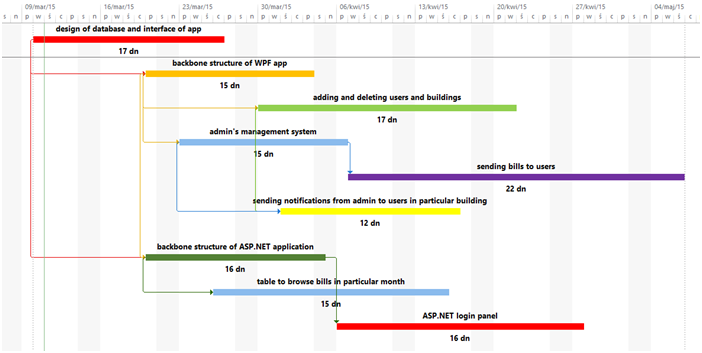
\includegraphics[width=1\textwidth]{img/gantt.png}
                \caption{Plan of work with exact dates in form of Gantt chart}
\label{fig:rys1}
\end{figure} 

\begin{itemize}
  \item \textbf{Design of database and interface of an application} 
  \newline Firstly there is a need to create design of datebase as a ERD diagram to implement it afterwards. In the same time interface of an application shoud be considered to be user-friendly, professional, easy and efficient. Interface of an application for users is especially important. For administrators it doesn't have to be that much spectacular. 

  \item \textbf{Backbone structure of WPF application} 
    \newline
     Then, a graphical subsystem for rendering user-interfaces in applications using Microsoft Windows called Windows Presentation Foundation is chosen and backbone structure of application is created. 

  \item \textbf{Adding and deleting users and buildings} 
    \newline These are very important features that should be applied, because the application is about users, buildings and bills. 

  \item \textbf{Admin's management system} 
    \newline It includes all bills that should be sent to users. There are some quotients inputed by admin such as cost per \(1m^2\) of water etc., amount of (for example) water used by particular residents, button to generate total amount of money and sending a bill via email or/and to user's application.

  \item \textbf{Sending bills to users} 
    \newline Sending bills to users by email, storing it in database, access by user to data via apllication.
  
  \item \textbf{Sending notifications from admin to users in particular building} 
    \newline Sometimes there is a need to send notification. For example resident have to be present at home in particular time because of water meter replacement and sending notification is more efficient than sticking announcement on a paper somewhere on the wall in the buildings. 
  
  \item \textbf{Backbone structure of application ASP.NET} 
    \newline Than server - side Web application framework designed for Web development to produce dynamic Web pages called ASP .NET is chosen and backbone structure of application is created.
  
  \item \textbf{Table to browse bills in particular month} 
    \newline There is a feature that help users to measure, manage and estimate the usage of for example water. 
  
  \item \textbf{Logging to application ASP.NET} 
    \newline This is a feature that includes users names and hashes of the passwords in database and system of logging to application. It allows to users identification, authentication and authorisation with the high level of security and personal data protection. 
\end{itemize}

\begin{table}[h]
\begin{tabular}{|l|l|l|l|}
\hline
\rowcolor{blue!30!}\textbf{Task name}&\textbf{Time}&\textbf{Start date }&\textbf{End date}            \\ \hline
design of database and interface of app                                                                     & 17 days               & tue, 10/03/15               & thu, 26/03/15             \\ \hline
backbone structure of WPF app                                                                               & 15 days               & fri, 20/03/15               & fri, 03/04/2015           \\ \hline
adding and deleting users and buildings                                                                     & 17 days               & mon, 30/03/15               & tue, 21/04/15             \\ \hline
admin's management system                                                                                   & 15 days               & mon, 23/03/15               & mon, 06/04/15             \\ \hline
sending bills to users                                                                                      & 22 days               & tue, 07/04/15               & wen, 06/05/15             \\ \hline
\begin{tabular}[c]{@{}l@{}}sending notifications from admin \\ to users in particular building\end{tabular} & 12 days               & wen, 01/04/15               & thu, 16/04/15             \\ \hline
backbone structure of ASP.NET application                                                                   & 16 days               & fri, 20/03/15               & sat, 04/04/15             \\ \hline
table to browse bills in particular month                                                                   & 15 days               & thu, 26/03/15               & wen, 15/04/15             \\ \hline
ASP.NET login panel                                                                                         & 16 days               & mon, 06/04/15               & mon, 27/04/15             \\ \hline
\end{tabular}
\caption{Plan of work with exact dates in form of table}
\end{table}



%%%%%%%%%%%%%%%%%%%%%%%%%%%%%%%%%%%%%%%%%%%%%%%%%%%%
%%%%%%%%%%%%%%%%%%%%%%%%%%%%%%%%%%%%%%%%%%%%%%%%%%%%
%%%%%%%%%%%%%%%%%%%%%%%%%%%%%%%%%%%%%%%%%%%%%%%%%%%%

\chapter{Project estimation}

Estimation process is important, but also difficult. In estimation of this product change of requirements and young age of team members will take great matter. Team members are inexperienced and for all of them this project is first on a big scale. Another issue of estimation for house cooperative software is fact that it's immaterial goods. WBS created below should help with estimation process - small tasks are much easier to estimate than whole software creation procedure. 

\section{Work breakdown structure}
As Gantt chart give a look for exact division of all implementation tasks. Presented below WBS (work breakdown structure) presents all tasks which have to be considered during all project procedures (from planning until maintaining).

 \begin{figure}[H]
    \centering
            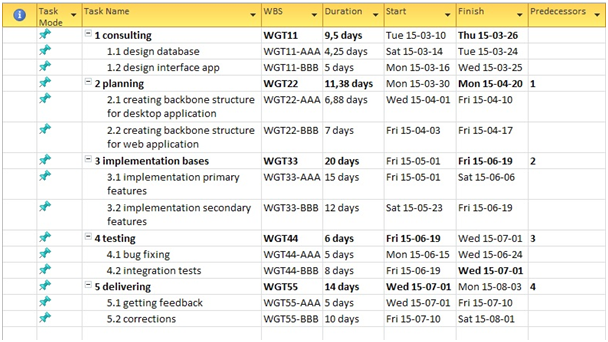
\includegraphics[width=1\textwidth]{img/WBS.png}
                \caption{Work Breakdown Structure in the table form and detailed plan of tasks realization}
\label{fig:rys1}
\end{figure} 

\begin{itemize}
  \item \textbf{Consulting} – contact with client to exchange information about technic aspects regarding costs and database’s speed and how interface should like.

  \item \textbf{Planning} – plan of the effort and time estimation. Moreover, creating backbone structures for desktop and web application. 

  \item \textbf{Implementation bases} – focusing on very primary requirements to enable implementation of secondary features. 

  \item \textbf{Testing} – however this project is based on Test Driven Development, at the end of the implementation process should be making some bug fixing and integration tests.

  \item \textbf{Delivering} – spending some time to give the software to the clients, getting feedback and making improvement. These tasks can be done parallely. 
\end{itemize}

\section{Function Points estimation}

It is not a big application so counting unadjusted function-point will be in small range. That's means that total weight in many factors will be having small parcel weights (in interval 1-3). Starting from functionality of software - It has to be considered - what exactly software has to be able to do. This functions are grouped in five categories (below table \ref{tab111}).

\begin{table}[H]
	\centering
\begin{tabular}{|l|l|l|}
\hline
\rowcolor{pink!80!}\textbf{Category}& \textbf{Multiplier} & \textbf{Weight} \\ \hline
External Inputs          & 3          & 2      \\ \hline
External Outputs         & 1          & 1      \\ \hline
External Inquiries       & 3          & 1      \\ \hline
Internal Logical Files   & 2          & 2      \\ \hline
External Interface Files & 2          & 2      \\ \hline
\end{tabular}
\caption{Function Points categories with complexity and weight of tasks}
 \label{tab111}
\end{table}

  \begin{enumerate}

 \item\textbf{Transactional Functions:}
   \begin{itemize} 
  \item \textit{External Inputs} - It stands for data collected as listed usage of gas, electricity, water and media bills in a database.
  \item \textit{External Outputs} - It is function of exportation data from application into pdf form.
  \item \textit{External Inquiries} - The system is requested for one thing, comined bill of usage electricity, whater etc.
  \end{itemize}
  
\item\textbf{Data Functions:}
  \begin{itemize}
  \item \textit{Internal Logical Files} - It is data collected from users (residents of house cooperative buildings) stored as tables with listed usage of gas, electricity, water and media bills in a database.
  \item \textit{External Interface Files} - Group of logically related data, in this project is content of database owned by house-cooperative web application. Residents data have to available for both sides (users and administrator).
  \end{itemize}  
 
  \end{enumerate}

To check how many functional points have created software, there is a need to multiply all transactional and data functions complexity (in \textit{Multiplier} column) by its weight for get FP of final product.

\[
FP = (3\ast2 )+(1\ast1)(3\ast1)+(2\ast2)+(2\ast2)= \textbf{18}
\]

After getting amount of functional points it is necessary to check how many hours in $C\#$ language is taken for each FP.  Some sources prove that one function point is an equivalent of eight hours of work in in $C\#$. There is a need of final multiplication to get needed amount of time.

\[
18\ast8 =  \textbf{144[hours]}
\]

\section{Detailed plan of realization and ProjectCodeMeter analysis}

Coding procedure will take approximatly 45 days.  The total work that should be done require about 61 working days:
\begin{enumerate}
  \item \textbf{Consulting} takes 9.5 days
  
  \begin{itemize}
  \item contact with clients
  \item calculating time and effort
  \end{itemize}

  \item \textbf{Planning} takes 11.38 days 
  
  \begin{itemize}
  \item creating backbone structures
  \item taking into account many implication and hard to predict tasks
  \end{itemize}
  
  \item \textbf{Implementation} takes 20 days 
 
  \begin{itemize}
  \item implementing e. g. admin’s management system, adding and deleting users and buildings,
	analysis of paying bills, account and database management

  \end{itemize}

  \item \textbf{Testing}  takes 6 days 
  
  \begin{itemize}
  \item integration tests and bug fixing using Sonar environmental
  \end{itemize}
  
  \item \textbf{Delivering} takes 14 days
  
  \begin{itemize}
  \item contact with client to get finish version of the software and getting feedback was went wrong
  \end{itemize}
  
  Any of tasks can start if and only if the last is ended. (For example planning can be started if consulting is done). It looks like waterfall, but providing Test Driven Development as well. This is an assurance, that there will be no reason to move back to the previous ones. 
  
\end{enumerate}



\begin{figure} [H]
\begin{subfigure}[b]{0.47\textwidth}
  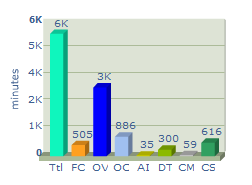
\includegraphics[width=\textwidth]{img/h.png}
  \label{fig:sub1}
\end{subfigure}%
\hfill 
\begin{subfigure}[b]{0.47\textwidth}
  \centering
  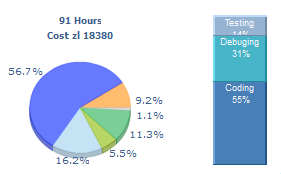
\includegraphics[width=\textwidth]{img/h2.png}
  \label{fig:sub2}
\end{subfigure}
  \caption{Cost and time estimation analized by ProjectCodeMeter}
  \label{fig:oba}
\end{figure}

\chapter{Risk Analysis}
\section{Risk Identification}

\begin{table}[H]
	\centering
\begin{tabular}{|l|l|l|l|}
	\hline
	\rowcolor{pink} \textbf{Root Cause} & \textbf{Condition} & \textbf{Consequence} &
	\begin{tabular}[c]{@{}l@{}} \textbf{Downstream}\\ \textbf{Effect} \end{tabular} \\

	\hline
	\begin{tabular}[c]{@{}l@{}} Bad project planning \end{tabular} &
	\begin{tabular}[c]{@{}l@{}} Project cannot be \\completed in time \\with given resources \end{tabular} &
	\begin{tabular}[c]{@{}l@{}} Necessity to employ \\another person  \end{tabular} & 
	\begin{tabular}[c]{@{}l@{}} Cost increase\end{tabular} \\

	\hline	
	\begin{tabular}[c]{@{}l@{}} Worker skills level/\\
		Bad project planning \end{tabular} &
	\begin{tabular}[c]{@{}l@{}} Employee can't complete \\
		task in given time  \end{tabular} &
	\begin{tabular}[c]{@{}l@{}} Other tasks may not \\ be able to start before \\ completing that one \end{tabular} & 
	\begin{tabular}[c]{@{}l@{}} Delay in project \\
		performance\end{tabular} \\
	\hline
	
	Random situation & 
	\begin{tabular}[c]{@{}l@{}} Employee is unavailable \\
		for some period of time\end{tabular} &
	\begin{tabular}[c]{@{}l@{}} Company will have \\ 
		to  work with \\ reduced personnel\end{tabular} & 
	\begin{tabular}[c]{@{}l@{}} Delay in project \\ 
		performance \end{tabular} \\
	\hline
	
	\begin{tabular}[c]{@{}l@{}} Worker skills level \end{tabular} &
	\begin{tabular}[c]{@{}l@{}} Employee can’t fully \\ 
		complete given task \end{tabular} &
	\begin{tabular}[c]{@{}l@{}} Some part of \\functionality  
		will not \\be implemented\end{tabular} & 
	\begin{tabular}[c]{@{}l@{}} Reduced project \\quality and \\customer\\ satisfaction\end{tabular} \\
	
	\hline
	\begin{tabular}[c]{@{}l@{}} Worker skill level \end{tabular} &
	\begin{tabular}[c]{@{}l@{}} Problems with \\implementation important \\parts of the system \end{tabular} &
	\begin{tabular}[c]{@{}l@{}} Bugs occurrence \\in the system\end{tabular} & 
	\begin{tabular}[c]{@{}l@{}} Customer \\dissatisfaction\\ Additional costs of \\ fixing \end{tabular} \\
	
	
	\hline
	\begin{tabular}[c]{@{}l@{}} Random situation/\\ Worker skills level\end{tabular} &
	\begin{tabular}[c]{@{}l@{}} Hardware or software \\is damaged \\(inappropriate usage, \\random situation)
		\end{tabular} &
	\begin{tabular}[c]{@{}l@{}} Necessity to buy \\or repair equipment \end{tabular} & 
	\begin{tabular}[c]{@{}l@{}} Cost increase  \end{tabular} \\
	
	\hline
	\begin{tabular}[c]{@{}l@{}} Technical problem \end{tabular} &
	\begin{tabular}[c]{@{}l@{}} Problem with system \\
		integration  \end{tabular} &
	\begin{tabular}[c]{@{}l@{}} Necessity implement \\changes 
		to project \end{tabular} & 
	\begin{tabular}[c]{@{}l@{}} delay in project\\ performance\end{tabular} \\
	
	\hline
	\begin{tabular}[c]{@{}l@{}} Worker skill level \end{tabular} &
	\begin{tabular}[c]{@{}l@{}} Information are not\\
		 properly secured \end{tabular} &
	\begin{tabular}[c]{@{}l@{}} Leak of information\end{tabular} & 
	\begin{tabular}[c]{@{}l@{}} legal responsibility \end{tabular} \\

	\hline
	\begin{tabular}[c]{@{}l@{}} Potential user \\ 
		interoperability  \end{tabular} &
	\begin{tabular}[c]{@{}l@{}} Future user don’t want \\
		to dedicate time for \\
		consulting requirements\end{tabular} &
	\begin{tabular}[c]{@{}l@{}} Problem with creating \\
		appropriate gui \end{tabular} & 
	\begin{tabular}[c]{@{}l@{}} Reduced user\\ satisfaction\end{tabular} \\

	\hline
	\begin{tabular}[c]{@{}l@{}} Media supply companies\\ interoperability \end{tabular} &
	\begin{tabular}[c]{@{}l@{}} Media companies don’t \\want to make available \\some of the user \\information  \end{tabular} &
	\begin{tabular}[c]{@{}l@{}} Not all bills \\are collected in\\ developed system \end{tabular} & 
	\begin{tabular}[c]{@{}l@{}} customer \\ dissatisfaction\end{tabular} \\
	\hline
\end{tabular}
\caption{Risk list}
\end{table}

Source of risk can come from scope, schedule, stakeholder expectations, internal dependencies, security, integration, interoperability, implementation challenges, but they can be considered more generally as a source connected with people, process, technology or environment.  Due to the fact that our company starts up in IT business, most of the events that may occur with negative impact on the project’s ability to achieve performance and goals, may come from the inexperienced team members in many domains. The other important fact is that our company has short period of time, it is 4 months, to complete the project. Every change to the schedule may results in crossing the deadline.

\section{Risk Management Plan}

The Project Manager has overall responsibility for managing project risk. To make team member aware of risk through all phases of the project are organised special scheduled project meetings related to that topic. Project team members are responsible on that meeting for reporting to the project manager about potential occurrence of risk situations. If any risk factors or event will occur during the project which needs immediate attention, it should be reported via email to the project manager. The project manager is responsible for determining whether any of the identified risk factors or events requires further increased attention. New risk will be included in the risk register. Each notification in the risk register includes following elements: description of the risk event; probability that event will occur; cost, quality or schedule impact. Depending on the probability of risk occurrence and overall impact to the project are considered two possible reactions: attempt to mitigate the chance of occurrence and contingency actions after appearance of the risk factor.

Risk assessment consists of two factors: probability of occurrence and estimation of the impact on project. Both are described by numerical values from 1 to 5, which are corresponded to the factors in the following way:

\begin{table}[H]
	\parbox{.45\linewidth}{
		\centering
	\begin{tabular}{|l|c|}
		\hline
		\rowcolor{gray} \multicolumn{2}{|c|}{ \textbf{Probability of Occurrence} }   \\  \hline                                                                                        
		\begin{tabular}[c]{@{}l@{}} \textbf{Definition} \end{tabular} & \begin{tabular}[c]{@{}l@{}} \textbf{Value} \end{tabular}     \\ \hline
		\begin{tabular}[c]{@{}l@{}} Frequent \end{tabular} & \begin{tabular}[c]{@{}l@{}} 5 \end{tabular}     \\ \hline
		\begin{tabular}[c]{@{}l@{}} Likely  \end{tabular} & \begin{tabular}[c]{@{}l@{}} 4 \end{tabular}     \\ \hline
		\begin{tabular}[c]{@{}l@{}} Occasional \end{tabular} & \begin{tabular}[c]{@{}l@{}} 3 \end{tabular}     \\ \hline
		\begin{tabular}[c]{@{}l@{}} Seldom \end{tabular} & \begin{tabular}[c]{@{}l@{}} 2 \end{tabular}     \\ \hline
		\begin{tabular}[c]{@{}l@{}} Improbable \end{tabular} & \begin{tabular}[c]{@{}l@{}} 1 \end{tabular}     \\ \hline
	\end{tabular}
	\caption{Probability of Occurrence}
	}
	\hfill
	\parbox{.45\linewidth}{
	\centering
	
	\begin{tabular}{|l|c|}
		\hline		\rowcolor{gray} 
		\multicolumn{2}{|c|}{  \textbf{Estimation of the impact}  } \\  \hline                                                     \begin{tabular}[c]{@{}l@{}} \textbf{Definition} \end{tabular} & \begin{tabular}[c]{@{}l@{}} \textbf{Value} \end{tabular}     \\ \hline                                   
		\begin{tabular}[c]{@{}l@{}} Catastrophic \end{tabular} & \begin{tabular}[c]{@{}l@{}} 5 \end{tabular}     \\ \hline
		\begin{tabular}[c]{@{}l@{}} Critical  \end{tabular} & \begin{tabular}[c]{@{}l@{}} 4 \end{tabular}     \\ \hline
		\begin{tabular}[c]{@{}l@{}} Moderate \end{tabular} & \begin{tabular}[c]{@{}l@{}} 3 \end{tabular}     \\ \hline
		\begin{tabular}[c]{@{}l@{}} Minor \end{tabular} & \begin{tabular}[c]{@{}l@{}} 2 \end{tabular}     \\ \hline
		\begin{tabular}[c]{@{}l@{}} Negligible \end{tabular} & \begin{tabular}[c]{@{}l@{}} 1 \end{tabular}     \\ \hline	
	\end{tabular}
	\caption{Estimation of the impact}
}
\end{table}

By adding those two numbers it is possible to compare importance of particular risks and focus on avoiding occurrence of the more important ones. The other ones with lower values are more acceptable and in that case will be taken steps to minimalize impact after occurrence. Risk with value 8 or more are considered as risks with highly importance, with value between 5 and 7 as risks with middle importance and with value lower or equal to 4 as a risk with low importance.


\begin{table}[H]
\begin{tabular}{|l|l|l|l|l|}
	\hline
	\rowcolor{orange}\ 
	\textbf{Risk}  & 
	\begin{tabular}[c]{@{}l@{}} \textbf{Overal} \\ \textbf{Impact}\end{tabular}  & 
	\textbf{Mitigation}   & 
	\textbf{Contingency} & 
	\textbf{CSP Impact}
	\\ \hline
	
	\begin{tabular}[c]{@{}l@{}} Employee is \\ unavailable for \\some period \\of time  \end{tabular} & 
	\begin{tabular}[c]{@{}l@{}}Minor + \\ Seldom = 4 \end{tabular}    & 
	\begin{tabular}[c]{@{}l@{}} In case of planned \\ and known earlier \\event, extension of \\worker time to \\overcompensate  later \\delays in schedule \end{tabular}                                                         &  \begin{tabular}[c]{@{}l@{}}  After consideration \\of importance of \\particular task \\being up-to-date \\with schedule, \\employ temporarily \\another employee \\or accept delay  \end{tabular} & 
    \begin{tabular}[c]{@{}l@{}}Delay in project \\performance,\\
    	Additional Cost \end{tabular} 
	\\ \hline
	
	\begin{tabular}[c]{@{}l@{}} Employee can't \\fully complete \\given task  \end{tabular} & 
	\begin{tabular}[c]{@{}l@{}}Moderate +\\Seldom = 5 \end{tabular} & 
	\begin{tabular}[c]{@{}l@{}} Appropriate \\preparation and \\ explanation of given \\task by project \\manager, spend \\some time on \\research \end{tabular}   & 
	\begin{tabular}[c]{@{}l@{}} Consult problem \\between co-workers\end{tabular} & 
	\begin{tabular}[c]{@{}l@{}} Delay in project\end{tabular}
	\\ \hline
	
	\begin{tabular}[c]{@{}l@{}} Employee can't \\complete task \\in given time  \end{tabular} &
	 \begin{tabular}[c]{@{}l@{}}Moderate +\\Occasional = 6  \end{tabular} & \begin{tabular}[c]{@{}l@{}} 
	 	Appropriate \\estimation of \\working hours \\needed to complete\\ the task\end{tabular}   & \begin{tabular}[c]{@{}l@{}} Assign other \\available worker \\to that task, \\employ another \\worker, if task not\\ influent other \\tasks accept delay \end{tabular} & 
	\begin{tabular}[c]{@{}l@{}} Additional cost \end{tabular}

	\\ \hline
		
	\begin{tabular}[c]{@{}l@{}}Media companies \\don’t want to \\make available \\some of the user \\information  \end{tabular} & \begin{tabular}[c]{@{}l@{}}Moderate +\\Seldom = 5  \end{tabular} & \begin{tabular}[c]{@{}l@{}} Earlier consultations \\about terms on\\ which media supply \\companies want \\to cooperate\end{tabular}   & 
	\begin{tabular}[c]{@{}l@{}} Try to renegotiate\\ agreement on\\ different terms\end{tabular} & 
	\begin{tabular}[c]{@{}l@{}} Reduced project\\ performance\end{tabular}
	\\ \hline
	
	\begin{tabular}[c]{@{}l@{}}Future users \\don’t want to \\dedicate time \\for consulting \\requirements  \end{tabular} & \begin{tabular}[c]{@{}l@{}}Moderate + \\Likely = 7 \end{tabular} & \begin{tabular}[c]{@{}l@{}} Find earlier \\a group of users \\that will dedicate \\time to consult \\requirements \end{tabular}   & \begin{tabular}[c]{@{}l@{}} Follow project with \\overall customer\\ requirements\end{tabular} & 
	\begin{tabular}[c]{@{}l@{}} Reduced user \\satisfaction\end{tabular}
	\\ \hline
	
	\begin{tabular}[c]{@{}l@{}}Information are \\not properly\\ secured\end{tabular} & 
	\begin{tabular}[c]{@{}l@{}} Catastrophic + \\Occasional = 8\end{tabular} & 
	\begin{tabular}[c]{@{}l@{}} Consult project with \\security specialist \end{tabular}   & 
	\begin{tabular}[c]{@{}l@{}} Try to repair \\damages and consult\\ with security \\specialist for \\further protection \end{tabular} & 
	\begin{tabular}[c]{@{}l@{}} Additional cost\\ delay in schedule\end{tabular}
	\\ \hline
	
	\begin{tabular}[c]{@{}l@{}}Hardware or \\software is \\damaged\\ (inappropriate \\usage, random \\situation)   \end{tabular} & \begin{tabular}[c]{@{}l@{}}Moderate +\\Seldom = 5  \end{tabular} & \begin{tabular}[c]{@{}l@{}} Instruct workers how \\to appropriate use \\an equipment, prepare \\documentation \\about configuration \\of environment to \\work with required \\software \end{tabular}   &
	 \begin{tabular}[c]{@{}l@{}} Buy or repair \\equipment \end{tabular} & 
	\begin{tabular}[c]{@{}l@{}} Additional cost\\delay in project \end{tabular}
	\\ \hline
\end{tabular}
\end{table}


%
%\bibliographystyle{plain}
%\bibliography{myBib}

\end{document}